\begin{XeClass}{Command}
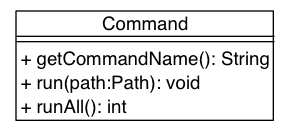
\includegraphics[width=\textwidth]{cdig/Command.png}
     
 用于执行文件命令的抽象类.

    \begin{XeMethod}{\XeAbstract \\ \XePublic}{String}{getCommandName}
         
 删除潜在的前导字符, 返回命令名 

    \end{XeMethod}

    \begin{XeMethod}{\XeAbstract \\ \XeProtected}{void}{run}
         
 在给定的路径上执行文件命令

    \end{XeMethod}

    \begin{XeMethod}{\XePublic}{int}{runAll}
         
 在给定的路径簇上的执行命令, 并返回状态码

    \end{XeMethod}

\end{XeClass}
